%!TEX TS-program = xelatex
%!TEX encoding = UTF-8 Unicode

\documentclass[12pt]{article}
\usepackage[a5paper,margin=2cm]{geometry}
\usepackage[french]{babel}
\usepackage{amssymb,amsthm,amsmath}
\usepackage{xltxtra}
\usepackage{stmaryrd}
\usepackage{graphicx}
\usepackage{listings}
\usepackage{color}
\lstset{
	extendedchars=false,
	showstringspaces=false,
	escapeinside=``,
	keywordstyle=\color{blue},
	commentstyle=\color[rgb]{0.133,0.545,0.133},
	columns=flexible,
	language=C++,
	tabsize=4,
	basicstyle=\ttfamily,
	numbers=left,
	frame=lines
}

\begin{document}
\tableofcontents\vspace{0.5cm}
\begin{center}
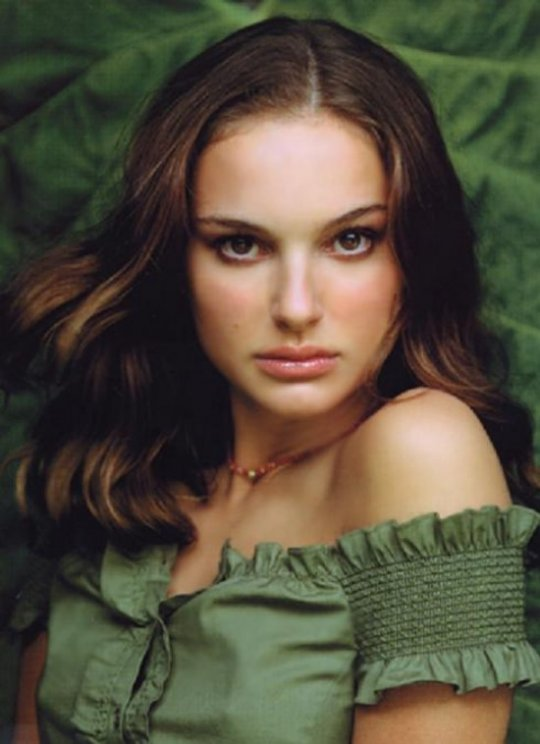
\includegraphics[width=0.8\linewidth]{np.jpg}
\end{center}

%\chapter{ACM Cookbook}
\section{Algorithmique du texte}

\subsection{Tableaux de suffixes}
Temps de cuisson : $O(n \log^2 n)$
{\scriptsize\lstinputlisting{code/suffix.cpp}}

\subsection{Knuth-Morris-Pratt}
Temps de cuisson : $O(n)$
{\scriptsize\lstinputlisting{code/kmp.cpp}}

\section{Optimisation}

\subsection{Sparse max-flow}
{\scriptsize\lstinputlisting{code/Dinic.cc}}

\subsection{Min-cost max-flow}
{\scriptsize\lstinputlisting{code/MinCostMaxFlow.cc}}

\subsection{Push-relabel max-flow}
{\scriptsize\lstinputlisting{code/PushRelabel.cc}}

\subsection{Min-cost matching}
{\scriptsize\lstinputlisting{code/MinCostMatching.cc}}

\subsection{Max bipartite matching}
{\scriptsize\lstinputlisting{code/MaxBipartiteMatching.cc}}

\subsection{Global min cut}
{\scriptsize\lstinputlisting{code/MinCut.cc}}

\section{Géométrie}

\subsection{Convex hull}
{\scriptsize\lstinputlisting{code/ConvexHull.cc}}

\subsection{Miscellaneous geometry}
{\scriptsize\lstinputlisting{code/Geometry.cc}}

\subsection{Slow Delaunay triangulation}
{\scriptsize\lstinputlisting{code/Delaunay.cc}}

\section{Algorithmes numériques}

\subsection{Number theoretic algorithms (modular, Chinese remainder, linear Diophantine)}
{\scriptsize\lstinputlisting{code/Euclid.cc}}

\subsection{Systems of linear equations, matrix inverse, determinant}
{\scriptsize\lstinputlisting{code/GaussJordan.cc}}

\subsection{Reduced row echelon form, matrix rank}
{\scriptsize\lstinputlisting{code/ReducedRowEchelonForm.cc}}

\subsection{Fast Fourier transform}
{\scriptsize\lstinputlisting{code/FFT_new.cc}}

\subsection{Simplex algorithm}
{\scriptsize\lstinputlisting{code/Simplex.cc}}

\section{Graphes}

\subsection{Fast Dijkstra's algorithm}
{\scriptsize\lstinputlisting{code/FastDijkstra.cc}}

\subsection{Strongly connected components}
{\scriptsize\lstinputlisting{code/SCC.cc}}

\section{Structures de données}

\subsection{Suffix arrays}
{\scriptsize\lstinputlisting{code/SuffixArray.cc}}

\subsection{Binary Indexed Tree}
{\scriptsize\lstinputlisting{code/BIT.cc}}

\subsection{Union-Find Set}
{\scriptsize\lstinputlisting{code/UnionFind.cc}}

\subsection{KD-tree}
{\scriptsize\lstinputlisting{code/KDtree.cc}}

\section{Divers}

\subsection{Longest increasing subsequence}
{\scriptsize\lstinputlisting{code/LongestIncreasingSubsequence.cc}}

\subsection{Dates}
{\scriptsize\lstinputlisting{code/Dates.cc}}

\subsection{Prime numbers}
{\scriptsize\lstinputlisting{code/Primes.cc}}

\end{document}